\documentclass[12pt,twocolumn,titlepage]{article}

%\usepackage[margin=.6in]{geometry} % set the margins to 1 inch on all sides
%\usepackage[left=25mm, right=25mm, top=15mm, bottom=20mm, noheadfoot]{geometry}

\usepackage{amsmath}
\usepackage[pdftex]{graphicx}
\usepackage{url}
\usepackage{titlesec}
\usepackage{relsize}
\usepackage{amsfonts}
\usepackage{fancyhdr}
\usepackage{amsmath}
\usepackage[boxed]{algorithm2e}
\usepackage{enumitem}
\usepackage[]{hyperref}
\setlist[enumerate]{itemsep=0mm}

\pagestyle{fancy}
\newcommand*{\justifyheading}{\raggedright}
\titleformat{\chapter}[display]
  {\normalfont\huge\bfseries\justifyheading}{\chaptertitlename\ \thechapter}
  {20pt}{\Huge}
 \titleformat{\section}
 {\normalfont\Large\bfseries\justifyheading}{\thesection}{1em}{}
\titleformat{\subsection}
{\normalfont\large\bfseries\justifyheading}{\thesubsection}{1em}{}
\usepackage[english]{babel}
\usepackage{blindtext}



\begin{document}
\begin{titlepage}
\thispagestyle{empty}

    \begin{center}
        
        \Huge
        \textbf{Unsupervised, Auto K-Means \\Audio Clustering\\using Dynamic Weight Selection} \\
        \vspace{0.5cm}
        \Large
        Jacob Elliot Reske
        \Large

        \vspace{1.5cm}
        
        \large
        in partial fulfillment of the requirements for the degree of\\
        \textbf{Bachelor of Arts, Music (INT)}\\
        at\\
        \textbf{Yale University}
        \large
        \vspace{5.5cm}
        
        
\includegraphics[width=0.25\textwidth]{yale}
        
        \Large
        \small
        Department of Music\\
        Yale University\\
        New Haven, Connecticut 06511 USA
        May 3, 2014
        \small
    \end{center}
\end{titlepage}


\textbf{\emph{Abstract} -- Fully unsupervised, automatic clustering by musical features (e.g. timbre, pitch, and rhythm) presents a number of problems. Selecting essential criteria for musical feature extraction, preprocessing the data, and finding similarities in the results introduces typical machine learning problems of overfitting and high dimensionality. The benefits of creating a fully unsupervised clustering algorithm, however, are clear. Fully unsupervised clustering could find unlikely matches in disparate musical styles, as well as a method to process large (or very new) datasets from streaming sources. Music researchers could use this tool to observe similarities in new, uncategorized, or recently digitized music (i.e. without ID3 tags). In this paper, we propose a toolkit that combines a robust musical feature selector and an auto-k, auto-weighted k-means clustering algorithm.}

\textbf{\emph{Index} -- unsupervised clustering, k-means, feature selection, Gaussian mixture models, dynamic weight selection, musical instrument recognition, Minkowski Weighted K-means, genre clustering.}



\section{Introduction}

For human beings, music conceptualization is a complicated and multi-layered cognitive process. Categorization is an essential means of distinguishing musical concepts, and it is one of the most preliminary cognitive acts associated with musical listening. \cite{Conceptualizing} An AI that can navigate musical concepts, then, must have some process equivalent to categorization-- placing instruments, songs, or artists in relation to similar music it has encountered before. Like humans, it must be able to construct a model of musical space-- based on the features of sound it thinks are important-- and relate new pieces of music to frameworks in that space. 

There are two ways to approach this problem, and they relate to two basic analytical frameworks in machine learning. \emph{Supervised learning} trains on subset of data where the categories are already known, building a model that can categorize future data based on earlier inferences. \emph{Unsupervised learning}, on the other hand, does not use pre-defined labels to construct its model. Its goal is to search for patterns already present in the training data and construct ways of conceptualizing this data further. Much has been written about supervised classification of music; instrument recognition \cite{Essid} and genre classification \cite{MaggbladeHongKao} \cite{LiChan} stand out as the largest problems in the supervised learning domain of music. Because our aim is to develop tools for categorizing music independently-- that is, independent of predefined labels-- we turn to unsupervised learning. A robust automatic clustering tool could be used to find patterns in a large, inter-generic corpus of music that would otherwise be apparent, or ones that normal genre categories might obfuscate. Extracting features based on the audio content itself (independent of metadata) could allow this algorithm to cluster unlabeled music, such as streaming audio, new music, or music in mediums and cultures with unstandardized meta-tags. Musicologists could apply these techniques to discover patterns in timbre, instrumentation, or rhythm that might be difficult to trace on a large corpus of music.

Like most other unsupervised learning problems, music clustering has three essential components. First, \emph{feature extraction} (\ref{sec:feature}) attempts to codify patterns of timbre, rhythm, and pitch in a quantifiable way. We propose three standard features to extract timbre, rhythm, and instrumentation: Mel-frequency cepstrum coefficients, octave band signal intensity, and amplitude modulation. Second, the \emph{preprocessing} step (\ref{sec:preprocessing}) eliminates noise, compresses the (usually large) data per song into feature vectors, and normalizes it for direct comparison. Finally, the \emph{clustering} phase (\ref{sec:clustering}) attempts to locate patterns when the songs are placed in feature space, creating dynamically-sized clusters that model the relationship from one song to another.

Fully automating the clustering step, however, presents some unique problems. Most unsupervised clustering algorithms still require some criteria to be specified beforehand, and picking good weights for all of the features used for clustering is difficult as the number of features increases. To solve this, we modify standard K-means algorithm to automatically choose a good cluster number $k$ and find optimal feature weights for every cluster before running the actual clustering step. in (\ref{sec:testing}), we present the results of auto-k and auto-weight algorithms with our music datasets, and in (\ref{sec:future}) we propose new heuristics to address these results.


\section{Feature Extraction}
\label{sec:feature}

The core component of any audio analysis method, the feature extraction phase attempts to quantify audio ``features'' as meaningful streams of analytical data. A wealth of literature on audio feature extraction already exists, detailing methods to extract information about timbre, pitch, rhythm, and energy of a given audio file. The issue, becomes one of curation: the features extracted must be both general enough to apply across a number of different musical styles and specific enough to convey meaningful information. Our feature extraction tool is a modified version of Yaafe, a Python library that can process and output 20 distinct features. \cite{yaafe} Our implementation can make use of any of them, but we will focus on three features whose traits prove salient in the genre problem: Mel-frequency cepstrum coefficients (MFCC), octave band signal intensity (OBSI), and amplitude modulation (AM). 

\subsection{Mel-frequency cepstrum coefficients}

Loosely defined, MFCCs attempt to approximate the timbral activity of a given sound or set of sounds. They attempt to represent an audio spectrum as a series of discrete frequency blocks-— a cepstral representation— each with their own spectral properties. In an MFCC transformation, each cepstrum is mapped onto the mel scale, a pitch scale designed to space spectral information so that, perceptually, pitches are spaced ``equally'' apart. Our algorithm for converting hertz ($f$) to mels ($m$) uses the formula in \cite{Speechcomm}: 

\begin{equation}\label{}
m = 2595 \cdot log_{10}(1 + f/700).
\end{equation}

The general technique for MFCC computation is as follows: first, the given audio signal is partitioned into windowed segments of width w (specified by the sample size). For each frame, we apply a Fast Fourier Transform. The signal is then converted to a Mel-warped spectrum using X, creating a modified time-frequency window on the mel scale. A triangular filter-bank is then applied directly on the resulting signal. Since they are uniformly distributed on the mel scale, each triangular windows is comparable from file to file. \cite{Essid} We then apply a Discrete Cosine Transformation (DCT) to the resulting log of each window's output to get an MFCC vector for that window. We use other techniques, such as spectral mean subtraction, to normalize the vector at this stage. The result is a spectral vector, and its amplitude is the MFCC value for that time and mel-frequency window. At this point, we can also use each MFCC coefficient matrix to create a new matrix of first and second time derivatives, and the lower rows of the new matrix are trimmed to give this new matrix the same shape as the original. 


Mel-frequency cepstrum coefficients are very popular when timbral extraction is needed, and much has been written about general MFCC's utility in speech recognition systems, instrument recognition, and genre classification. However, until recently, MFCCs were considered invariant to other extra-timbral features, such as tempo and key. In their paper,``Genre classification and the invariance of MFCC features to Key and Tempo,'' Tom Li and Antoni Chan suggest that MFCC data does incidentally encode tempo and key information, and that songs performed in atypical keys/tempi were less accurately classified than those with typical traits. What's more, their findings suggest that genre classifiers, like the genres that they model, ``are in fact influenced by the fundamental keys of the instruments involved,'' despite the common intuition that key does not influence genre. \cite{LiChan} We will explore this postulation in our own results section (\ref{sec:testing}).

\subsection{Octave band signal intensity}

While MFCCs encode timbral information by splitting the spectrum into discrete time-frequency bands, there is merit in capturing timbral information in other ways. Octave band signal intensity (OBSI) attempts to describe the power distribution of an instrument or set of instruments by splitting it into octave sub-bands. 


The process is similar to the MFCC computation. For each time step, We partition the subset of the spectrum that contains normal musical notes (A0 at 27.5Hz to A8 at 7040.00Hz) into octaves using a triangular filterbank. Each octave band is calculated by multiplying frequencies in the usual manner, using the An frequencies as edges. We use triangular filters to force different distributions for two instruments that inhabit the same octave band. We then calculate the log of the energy spectral density in this octave band, and define the energy spectral density $E$
 by the formula: \cite{Oppenheim}

\begin{equation}\label{}
E = log\left(\int_{-\infty}^{+\infty} \mathrm{|x(t)|}^2\, \mathrm{d}t\right) \; \text{for time-series} \; x(t).
\end{equation}

As with MFCCs, the frequency band is standardized by octaves, so the columns of the resulting matrix are comparable from file to file. We also can compute the log ratio of the first band's energy with each subsequent band to get a matrix of OBSI ratios (labeled OBSIR). The general algorithm for OBSI feature extraction is described in \cite{Essid}. While not as useful for more timbrally complex pieces of music, this feature is especially useful for encoding the differences in power spectrum between instruments or a group of instruments. Below, we reproduce the graph of octave band signal intensity found in \cite{Essid}, comparing the spectra of an alto sax and Bb clarinet.
%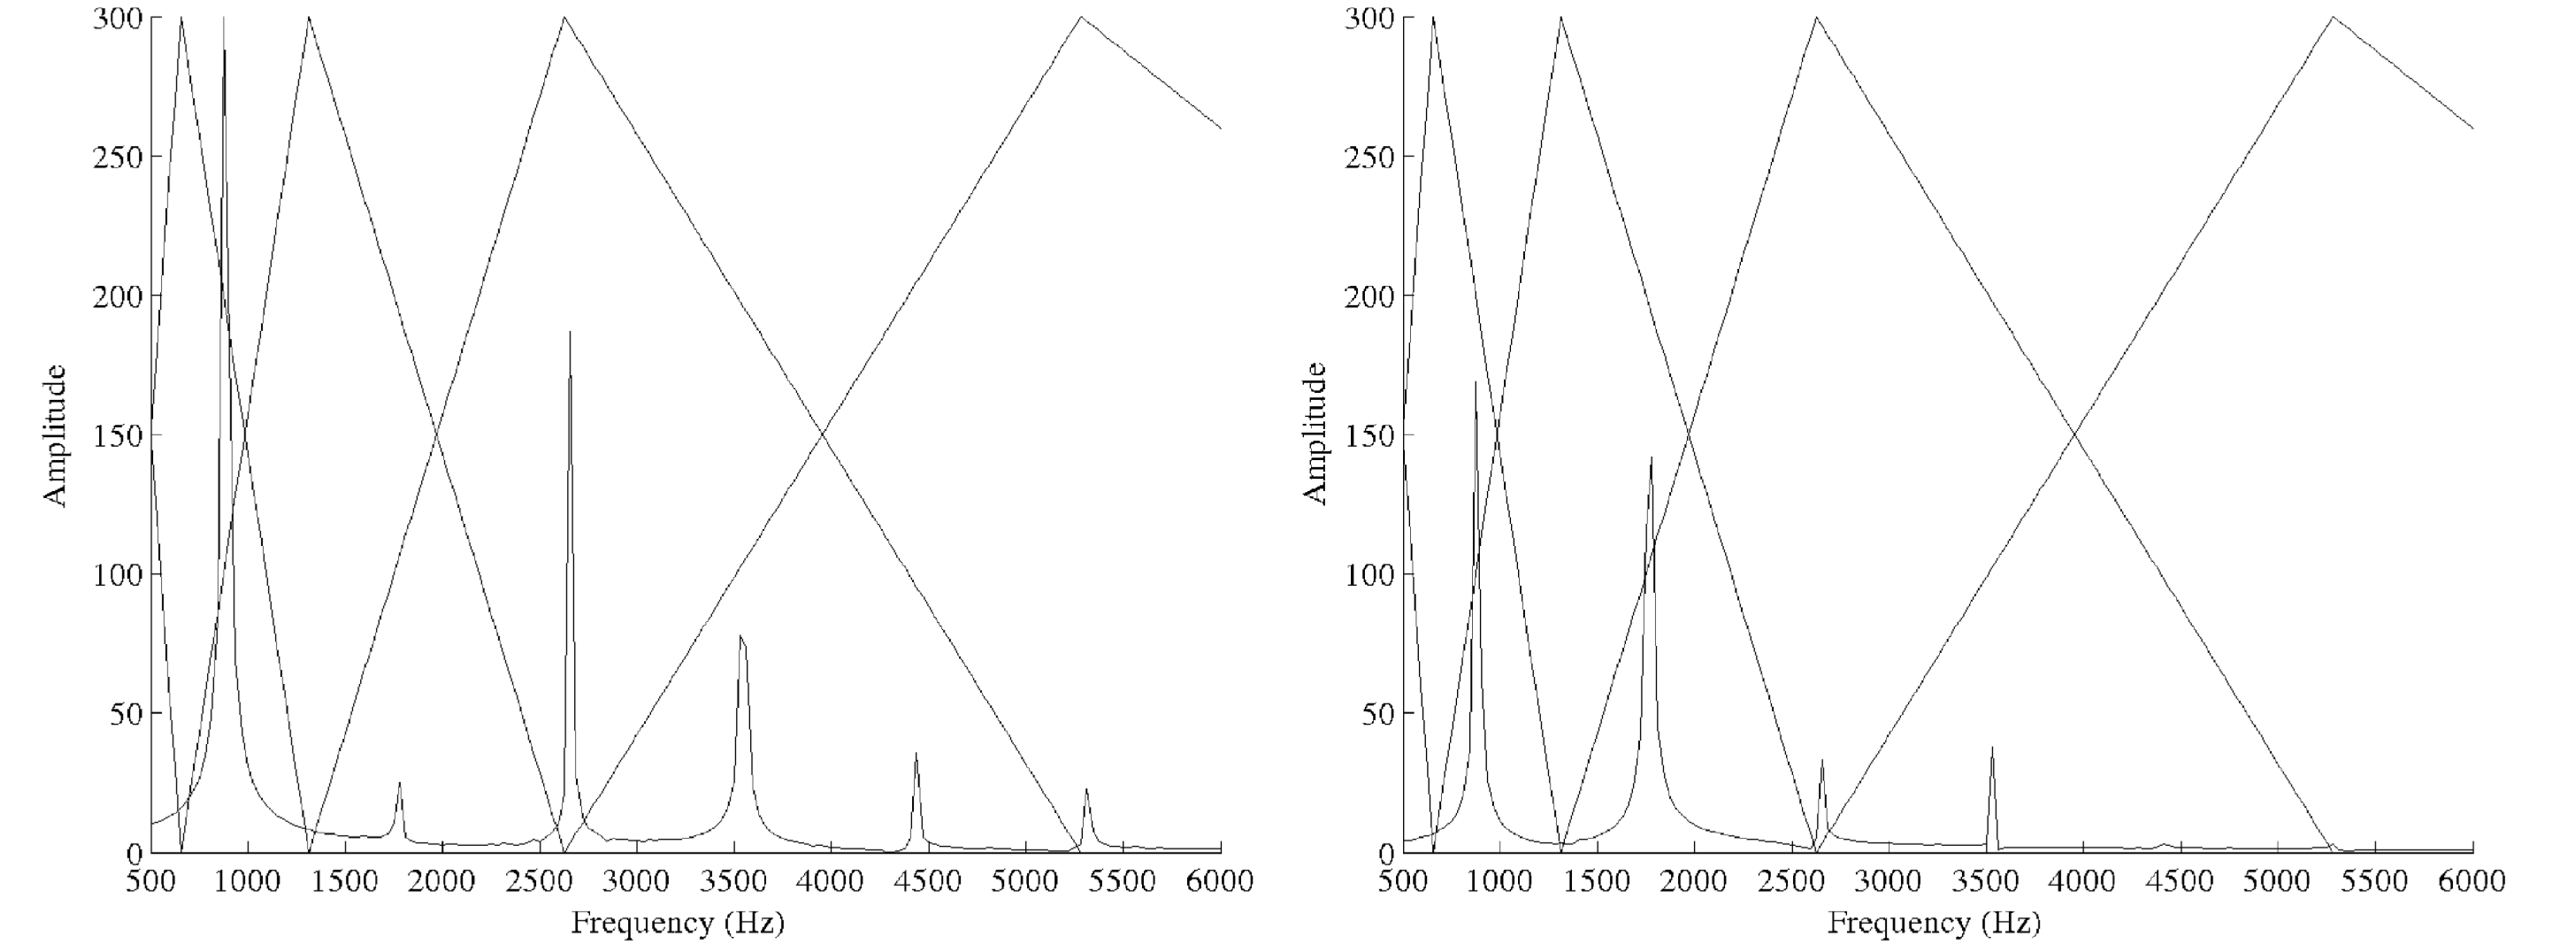
\includegraphics[width=.5\textwidth]{obsi}
\subsection{Amplitude Modulation}

Amplitude modulation attempts to encode two values: the average pitch displacement given constant amplitude (\emph{tremolo}) and the average amplitude displacement given constant pitch (\emph{grain}). \cite{Eronen} For each spectral fame, a modulation of 4 -- 8Hz in tremolo and 10 -- 40Hz for grain are recorded an analyzed. For  each range, the maximum energy is found, and the difference between this and the mean energy in this range is computed. \cite{yaafe} The product of these two values represents the amplitude modulation in this time-frequency range.


\section{Preprocessing}
\label{sec:preprocessing}


\subsection{Mean/covariance pairs}

As described in (\ref{sec:feature}), each feature extraction method in the process produces a matrix in $\mathbb{R}^2$ with a high dimension. Since each feature is processed by time step (in our algorithm, the default step size is 256 samples) and thus is composed of n sparse vectors, the resulting matrices are unsuitable for direct comparison. The MFCC extractor, for example, returns an $m\times13$ matrix, where $m \sim 8600$ for a 5:00 minute file. 


To remedy this, a sample mean and variance-covariance pair is computed for each set of vectors. We use the standard formula for computing variance-covariance: the mean vector preserves the average value for each column (in the MFCC case, the log spectral partition). The variance-covariance matrix preserves the variances of variables $i$ in position $(x_i, x_i)$, and the covariance between values $i, \;j$ in position $(x_i, x_j)$. The formula for covariance $\mathrm{C}$ is given as:

\begin{equation}\label{}
\mathrm{C} = \sum_{i=1}^{n}{\frac{(X_i-\overline{X})(Y_i-\overline{Y})}{n-1}}.
\end{equation}


and the formula for the mean vector is intuitive. This computation achieves two goals: it standardizes the dimensionality of each file's feature matrix, and it reduces dimensionality so computation is manageable. Computation time for later steps is reduced by limiting the number of compares required. The resulting matrices are stored in the current cluster's \texttt{FeatureSet} object for later use.

\subsection{KL-Divergence}

Next, we need a reliable method to represent the ``distance'' between two mean/covariance pairs. Any number of norms could be used on the covariance pairs $|X - Y|$, or any number of $L_i$ norms $i \in \{1,...,\infty\}$ (SEE PAGE BELOW), but the mean vector would be disregarded. We therefore consider feature vectors $x_1$, $x_2$ as multivariate normal (Gaussian) distributions modeled by means $(\mu_1, \mu_2)$ and covariance matrices $\Sigma_1, \Sigma_2$, and compute the Kullback-Leibler divergence between distributions. This represents the difference between normal distributions $\delta_1$ and $\delta_2$ \cite{ChiRussel-web}; Information Theory terms this information gain (entropy) between a two probability distributions, one of which is ``true'' or accurate. In terms of our .mp3's MFCC vectors, this represents the difference in probability distribution between a given song's calculated timbre and one that is close in timbral space. A KL-divergence test between an .mp3's MFCC feature vector and the same .mp3, then, should return a distance of 0. The formula for KL-Divergence between distributions $\delta_1$ and $\delta_2$ is given as:

\begin{equation}\label{}
\mathrm{D}_{KL}(\delta_1||\delta_2) = \sum_{x \in \delta}{}{\delta_1(x) \cdot log(\frac{\delta_1(x)}{\delta_2(x)})}.
\end{equation}

and, in terms of our normal distributions $X_1$ and $X_2$ and mean/covariance pairs $(\mu_1, \mu_2)$ and $(\Sigma_1, \Sigma_2)$:
\begin{multline}
\mathrm{D}_{KL}(\delta_1||\delta_2) = \frac{1}{2}\bigg(tr(\Sigma_2^{-1}\Sigma_1) + (\mu_2-\mu_1)^T \\
 \cdot \sigma_2^{-1}(\mu_2-\mu_1)-k-ln(\frac{det\Sigma_1}{det\Sigma_2})\bigg).
\end{multline}

Taken to an arbitrary power to preserve accuracy, this gives us an integer that represents the distance between a ``true'' song and another, as represented by probability distributions X1 and X2. However, unlike most distance calculations, KL-Divergence is asymmetric; $\mathrm{D}_{KL}(\delta_1 || \delta_2) \neq \mathrm{D}_{KL}(\delta_2 || \delta_1)$. Multiple methods of overcoming this (e.g. calculating resistor-average distance) \cite{JohnsonSinaovic} have been discussed. For our implementation, we divise a simpler solution by creating a (trivially) symmetric KL-Divergence, \cite{MaggbladeHongKao} labeled $\mathrm{DS}_{KL}$: 

\begin{equation}\label{}
\mathrm{DS}_{KL}(\delta_1, \delta_2) = \mathrm{D}_{KL}(\delta_1 || \delta_2) + \mathrm{D}_{KL}(\delta_2 || \delta_1).
\end{equation}


We compute $\mathrm{DS}_{KL}$ for all files in our \texttt{FeatureSet} manifest object (a list of all .mp3's to be processed). To speed our later clustering step, a general $nxn$ Divergence matrix (DIV) is created for each feature for $n$ .mp3 files, where $\mathrm{DIV}(x_i, x_j) = \mathrm{DS}_{KL}(x_i, x_j)$. This matrix should always adhere to a few requirements: $\mathrm{DIV}(x_i, x_i) = 0 \; \forall i \in N$ (the ``distance'' in feature space between an .mp3 and its duplicate should be zero), and $\mathrm{DIV}(x_i, x_j) = \mathrm{DIV}(x_j, x_i)$ (trivially, the Symmetric KL-Divergence should be symmetric). A simple check function is implemented at the end of the DIV matrix calculation to issue warnings and recompute if these requirements are not met. The resulting matrix is then stored in our FeatureSet object, and the process is done for every feature in \texttt{FeatureList}. If more features are introduced later in the processed and a DIV matrix was not computed, a new matrix will be added and recomputed. 

\subsection{Normalization}

One additional (optional) step is added here before clustering can begin: normalization across dimensions. Because each audio feature is independent and operates on different scales, the relative mean values of these feature vectors can vary drastically from feature to feature. The MFCC's average distance values, for example, might be several powers greater than other features' distances (such as AM or OBSI), skewing our clustering algorithm naturally in favor of the former's computed distances. To remedy this, we normalize each DIV matrix by dividing each entry by that matrix's infinity-norm, or the maximum of each of the row sums. \cite{Rudin} This normalization method is inherently rough, but it suits our purposes by scaling each feature's distances to be comparable.

\subsection{Summary}

To summarize: this process standardizes the feature vectors and prepares them for clustering by considering them as multivariate normal distributions. It computes the KL-Divergence (``distance'') values between .mp3 files and stores them for easy retrieval later. This preprocessing step drastically reduces the compute time of the clustering step, which references these distance values constantly.


\section{Clustering}
\label{sec:clustering}

\subsection{Basic K-means overview}

Now that we have distance values between all songs in our dataset, we can begin to cluster these songs into different, dynamically-sized categories. All of the algorithms proposed are variants on the standard K-means algorithm, so it is worthwhile to review the basics of this approach. K-means clustering is widely used for both its simplicity and applicability to a large variety of use cases—- from small to large dataset sizes, cluster count, and dimensionality. It is also a speedy algorithm and can be parallelized, making it optimal for our use case.


However, the K-means algorithm does not come without distinct disadvantages.  The most obvious disadvantage is that a fixed number of clusters k must be specified before the algorithm runs, requiring a level of guesswork and data snooping to get the right amount. Outliers also pose a problem; in the basic implementation, no data point is left out, and a few outlier points can quickly reduce the number of usable clusters. \cite{Sing} Thus, in its most basic form, K-means is not always suitable; the problem of song clustering should have different requirements and heuristics to overcome the algorithm's pitfalls. We therefore propose a number of improvements to the basic K-means algorithm for our use case— some of them implementations of existing research, others our original algorithms and heuristics. It is beyond the scope of this research to present an ``optimal'' variant of K-means for generalized music clustering. Our hope is to implement several variations and document their strengths and pitfalls in the context of the aforementioned genre problem.

The K-means algorithm is an evolutionary clustering algorithm that groups n  objects into a specified k number of clusters. Every K-means implementation has four steps that represent the core of the algorithm. They are below:

\begin{algorithm}
 \caption{\texttt{KMeans}}\label{algoCPOR}
 assign points in $\mathbb{R}^n$ as the centroids of k initial clusters.\;
 \While{$|C - C'| \neq 0$}{
  C' = C\;
  \For{$i\leftarrow x_1 \; \KwTo\ \; x_n$}{
   \For{$j\leftarrow k_1 \; \KwTo \; k_n$}{
    compute the distance $\mathrm{d}(v_i, x_i))$\;
    }
    assign $x_i$ to $\mathrm{min}(\mathrm{d}(v_i, x_i))$\;
   }{
  }
  recompute all centroids in C'\;
 }
 \KwRet final cluster configuration\;
\end{algorithm}

In \textbf{4)}, the threshold condition is usually related to the ``inertia'' of each cluster's centroid— how far it moves in feature space— from round to round. Depending on the dataset's size and sparseness, a cluster can take anywhere from 2-3 to hundreds of rounds to properly settle. Our input dataset never contains more than 600 songs, and the distance metric to centroids is implicit, so we have opted to hard-code a round maximum of 40, in the interest of simplicity. However, in our tests, we have found that even optimal k-sized clusters take significantly fewer than 40 rounds to stabilize. 

\subsection{Our implementation}

To accommodate our data, a few basic changes had to be made for our K-means implementation. Our \texttt{FeatureSet} object has computed distances between every song in all dimensions, but representing these features as sets of Gaussian distributions does not allow these songs to exist as points in any discernible feature space. We only have KL-Divergences that relate feature vectors to each other; this keeps us from computing an explicit $n$-dimensional centroid ``point.'' \cite{MaggbladeHongKao} proposes a solution: defining the centroids of each cluster implicitly, preserving the distance between centroid and point $x$  while eschewing a concrete value for the centroid. Formally, the distance between centroid $C$ and point $y$ is defined as:

\begin{equation}\label{}
\mathrm{D}(C, y) = sum_{i \in N}{}{\mathrm{D}(y, x_i) / n} \quad \forall x_i \in X_c.
\end{equation}

The distance function between xi and xj in $\mathbb{R}^n$ is also optimized to support a large dimension of disparate musical features. Since songs can be very metrically similar on one feature dimension but very different on another, picking a proper metric is very important. The most basic distance metric— Euclidean distance FIX THIS FIX THIS FIX THIS FIX THIS and it is most effective with features that have comparable scales (such as $\mathbb{R}^n)$. \cite{glynn} Other metrics weight dominant distances more or less prominently: the Manhattan Distance (1-norm), for example, simply takes the sum of the respective dimensional distances. Formally, the general formula for the p-norm is:

\begin{equation}\label{}
\|x\|_p = (\sum_{i=1}{n}{|x_i}^p)^{1/p}.
\end{equation}

In other literature, this  generalized form is called the Minkowski distance. \cite{Meyer} As p increases, the metric will become naturally biased toward dimensions with dominant (greater) distances; the infinity-norm, for example, is simply the max value of all distances. Choosing a proper p-value, then, represents how much we would like clusters to form based on the dominance of a single feature versus the even distribution of all features. Our current approach allows for a p-value to be input manually for each cluster; future versions of this algorithm will include a method to calculate an optimal p-value, much like the implementation in R's library. \cite{pvclust}

\subsection{Heuristics}

A few heuristics have been implemented to address some of K-means' inherent pitfalls. The random selection of initial centroids, for example, can easily derail a clustering job if the centroids are suboptimal. If the optimal centroids are, by definition, the final centroids of the k clusters, the initial points should not be too ``close'' to each other, relative to the size of feature space. This could unfairly exclude outlier clusters, all while dividing more central clusters along seemingly arbitrary lines. To remedy this, a distance heuristic is used to evenly distribute the initial k clusters. \cite{Zerbst} Once k random points are picked, the distances $\mathrm{D}(k_i, k_j)$ are checked against the average distance of all points $(xi, xj) \in X$ on every dimension. If any pair of centroids is closer than the median distance on that dimension, the cluster resets and reinitializes the centroids. This initialization process can take hundreds of tries for larger datasets, but (since all these values are stored) the compute time is largely negligible. Planned for future versions is a minimum distance, so that outliers do not dominate the list of initial centroids. A more practical solution, of course, may be to prune outliers entirely (discussed below).


A second solution to this problem is implemented on the other end; to prune bad initial centroids, we implement an iterate function in our \texttt{ClusterFactory} object to run the same cluster job a proportion of times related to the number of $n$ points. For each iteration, we store the final clustering in a dynamic stack to compare later. A simple sort is performed on the final clustering before the \texttt{push()} to make multiple results comparable, since K-means does not guarantee that clusters will be sorted the same way each time. After the cluster iterates, the stack is emptied, and the final clustering with the highest frequency over all iterations is recorded. This is considered the final, definitive clustering, removing outlier results from the solution. Instead of an automatic iteration count, a manual iteration value can be specified in the interface if the automatic value is insufficient or too computationally expensive.

\subsection{Auto-weighted k-means}

While the above tactics provide safeguards against outliers in both initialization and results— essentially by brute force— they do not address some of the limitations inherent in the K-means algorithm. As mentioned in I), a weighted implementation of K-means requires weights to be assigned beforehand. Picking optimum weights before testing based on those criteria invokes the hazard of assuming that these weights are optimum for the test set before testing has even begun. Testing a wide range of weight hypotheses and finding an making statistically inferences too quickly, on the other hand, can result in data snooping: making spurious or statistically insignificant correlations after the fact.


However, there is definite merit in using a heuristic on K-means to measure the optimum weight strategy, especially in datasets with many features. At high dimensions, n-dimensional space appears homogeneous \cite{KumarErtoz}.  Small correlations in one dimension (or subset of dimensions) can be outweighed by the relative homogeneity among the rest. To solve this, we consider the idea of cluster-specific weights. This stems from intuition about the nature of musical genres' criteria: one genre of music may be more dependent on a specific subset of features as its defining elements. While some genres are practically defined by instrumentation— the instruments in a Jazz combo, for example— other genres may cluster more predictably based on a specific tempo. 


To that end, we propose a set of heuristics built into the standard K-means algorithm, in an object labeled \texttt{KMeansHeuristic}. In addition to rounds, K-means is broken up into clusters. First, for n dimensions a list of $W$ possible even weights are computed, where each weight $w \in W$ (the total number of even weights) is contains $0 \leq i \leq n$ nonzero weights of the same value $v$, and $v*i = 1$. For $n = 3$, for example, the list of subsets 
is represented by the columns of matrix $\mathrm{M}$:

\begin{equation}\label{}
\mathrm{M} = \begin{bmatrix}
1 & 0 & 0 & .5 & 0 & .5 & .33 \\
0 & 1 & 0 & .5 & .5 & 0 & .33 \\
0 & 0 & 1 & 0 & .5 & .5 & .33
\end{bmatrix}.
\end{equation}

Each cluster then simulates the outcome of the coming round as if every cluster played one of the following weights, and plays the ``best'' weight for that round. For each cluster, the ``best'' weight is defined by the weight that gives the least Squared Error Distortion. Let $V = {v_1,v_2,...,v_n}$ be the set of n data points and $X$ be the set of centroids. Then $\mathrm{d}(vi, X) = \mathrm{min}(\mathrm{d}(v_i, x_i))\: \forall \: x_i \in X$. The Squared Error Distortion is given by the formula 

$$
\mathrm{d}(V,X) = \sum_{i=1}^{n} \frac{\mathrm{d}(v_i, X)^2}{n} \quad \forall v_i \in V.
$$

After each cluster has picked its optimal weight, the round is run in full, with distances calculated using the chosen weights for each cluster. A pseudocode illustration of this algorithm is given below:

\begin{algorithm}
 \caption{\texttt{KMeansHeuristic}}\label{algoCPOR2}
 Compute a list $W$ of the total number of even subsets of $w$, as defined in $X$\;
 \For{round $r\leftarrow 1 \; \KwTo\ \; R$}{
  Create array $A$\;
  \For{cluster $c\leftarrow 1 \; \KwTo\ \; C$}{
   \For{weight $w$ in $W$}{
    Run one round of K-means with all clusters $c \in C$ playing $w$\;
    $A[w] = min(\mathrm{d}(V,X))$\;
    }
   }
  Run round $r$ proper, where the distance from point $x$ to cluster $c$ is computed using the corresponding weight $w'$ associated with $c$.\;
 }
 \KwRet cluster configuration $C'$\;
\end{algorithm}

\texttt{KMeansHeuristic} can be combined with any of the above variations, such as multiple iterations and initial-point pruning, as its method is contained to a single round of K-means.

\subsection{Finding the best k}

Another basic limitation of the basic K-means algorithm is that—- naturally—- the number of clusters $k$ has to be specified beforehand. This can be necessary or useful in some cases— for example, sorting a list of $n$ songs into $k$ pre-specified genres— but it is not ideal for situations where the nature of the music being analyzed is not yet known. Furthermore, our goal for this algorithm (as mentioned in \ref{sec:feature}) is to find musical similarities in songs that may or may not be expected— ones that may require more or fewer clusters than the intuitive number. 


To account for this, we implement an auto-k method to determine and implement a clustering using the optimal k-value. As with our auto-weights implementation, our auto-k uses Squared Error Distortion (SQE) as a heuristic for determining how uniformly the cluster's points convene around a given centroid. This is run for $k: 1 \leq k \leq \log{n} / 3$, a value determined through testing to give a good range of possible $k$ values. The pseudo-code for our auto-k implementation is below: 

\begin{algorithm}
 \caption{\texttt{Auto K-means}}\label{algoCPOR3}
 Create array $A$\;
 \For{$k\leftarrow 1 \; \KwTo\ \; int(log(n)/3$}{
  \For{cluster $c$ in $C$}{
   Find SQE Distortion $\mathrm{d}(c,X)$\;
   }
  $A[k] = \sum_{c = i}^k{\mathrm{d}(c,X)} / k$\;
  }
 $k'$ = maximum value of array $A$\;
 Run \texttt{KMeans} using $k'$.
\end{algorithm}

As with other applications of Squared Error Distortion, our auto-k heuristic is greatly determined by the p-value chosen to measure the Minkowski distance from point to cluster. A higher p-value (such as the infinity norm) will weigh distortion more heavily in favor of clusters that group tightly in any one dimension. Choosing a proper p-norm is a machine learning problem in itself; our algorithm uses a semi-supervised method for finding an optimum p as described in \cite{SemiSupPNorm}. This method, however, requires a small portion of labeled data to find the p-value that ensures the best cluster, which defeats the purpose of making a fully unsupervised, auto-k algorithm. However, tests with supervised data and variable p on various datasets suggest that $p = 3$ is near optimal for most distortion cases. Unsupervised methods for finding an optimum p have been proposed, \cite{SemiSupPNorm} but they are beyond the scope of this research to implement. 

Like our first optimization, auto-k can be run with other heuristics, such as multiple iterations and initial-point pruning. 


\section{Testing and Results}
\label{sec:testing}


In this section, we will consider performance of both feature selection and variants on weighted k-means clustering on a number of different datasets. Our implementation, \texttt{MUS490}, is designed to work on any song dataset of any style or genre with little preprocessing. However, to test the algorithm's effectiveness ourselves, we prepared six distinct datasets of various styles and utility for testing. They are:
\begin{enumerate}[itemsep=0mm]
\item{\texttt{5Albums}, a dataset of five popular music albums released in 2013}
\item{\texttt{600Songs}, a dataset of 600 .mp3 files selected at random from the author's music collection}
\item{\texttt{Beatles}, the complete discography of the Beatles}
\item{\texttt{ClassicalPiano}, a collection of solo piano works by four Classical and Romantic composers (Bach, Mozart, Chopin, and Rachmaninoff)}
\item{\texttt{Jazz1959}, five albums by Jazz musicians released in 1959 (Bill Evans, John Coltrane, Miles Davis, Ornette Coleman, and Dave Brubeck)}
\item{\texttt{Instruments}, a custom sample library by Open Path Music, made available for the One Laptop Per Child project} \cite{OpenPathMusic}
\end{enumerate}

In the interest of replicating this data, manifests of each of these datasets' files (with metadata) will be made available upon request. In this section, we will consider the performance of \texttt{MUS490} in three separate context: instrument/ensemble identification, genre partitioning, and wild-card/unlabeled clustering. Unless noted otherwise, each section's tests is ordered by increasing difficulty. The most representative results for each of the tests are given in \texttt{<name>.log}, in the \texttt{logs} folder of the program.

\subsection{Instrument and ensemble identification}

\emph{test1\_1}: Our first test is a 2-cluster split of the \texttt{ClassicalPiano} dataset, with the hopes that \texttt{MUS490} splits by instrument type. (The Bach examples are recorded with a harpsichord, while the other three composers' works are played on piano). We run a 2-cluster test using equally weighted MFCCs, along with their first and second derivatives, and iterate until a result is seen at least three times. The results are consistent: \texttt{MUS490} successfully splits into one cluster of harpsichord and one of piano. Closer inspection of the saved divergence matrices confirms that the MFCC divergence is comparatively high for piano/harpsichord pairs. A similar run with the auto-k optimization enabled successfully selects $k = 2$ before splitting into the same cluster as above.

\emph{test1\_2}: In this test, we introduce our auto-k algorithm on the entire piano dataset, one which (minus the Bach) is fairly homogeneous on a timbral scale. Despite this, a low p-value is given to induce a higher cluster count, and auto-k splits the dataset into nine clusters with only MFCC data. Precision is high, but (due to the high k-size) recall is low, if artist-splits are the intention; Only a few Rachmaninoff examples are mis-clustered, and those the slower etudes and along with Chopin's nocturnes. The auto-k example reveals something new, however: a startlingly accurate split of the Mozart and Rachmaninoff examples by tempo. With Mozart, for example, we are left with three clusters: one of \emph{allegro} / \emph{presto} movements, one \emph{allegro} / \emph{allegretto}, and a third \emph{andante} / \emph{largo}. This experimentally confirms experimental results in \cite{LiChan} that find evidence of tempo encoding in normal MFCC vectors.

\emph{test1\_3}: We run a harder test using \texttt{Instruments} as our test set, once with a fixed set of three and four clusters (one for each instrument group) and once with auto-k clustering. Our first two tests uses even weights for the initial clustering, but other tests weighed OBSI or AM features more heavily than traditional MFCCs.

Our results show reliable clustering of string instruments (guitar, banjo, and bass) in all three examples. The low fixed-k examples of $k=3$ and $k=4$, however, introduces the larger outlier problem clearly: The clavinet and organ groups were distinct enough to deserve their own cluster, yet small enough to force relatively closer groups (e.g. keyboards and strings) to cluster together. Our auto-k algorithm picks $k=5$, giving brass/wind instruments their own partitions. Overall, each test is categorized by poor-to-moderate precision and good recall, an expected consequence of the outlier problem.

\subsection{Genre partitioning}

\emph{test2\_1}: We do a 3-cluster split of both the \texttt{ClassicalPiano} and \texttt{Beatles} datasets with five equally-weighted features (MFCC, MFCC\_d1, MFCC\_d2, OBSI, and AM), and results are predictably consistent. Recall is very high; only three of the 338 songs are ``mis-categorized'' on generic lines (predictably, three of the orchestral tracks from the ``Yellow Submarine'' album). When performed with a 2-cluster split, however, the Bach sub-cluster merges with \texttt{Beatles}. An auto-k version of this test (predictably) divides the clusters further, an expected result as the initial $k=3$ split is somewhat forced.

\emph{test2\_2}: Next is a 4-cluster split of \texttt{ClassicalPiano}, \texttt{Beatles}, and \texttt{Jazz1959} using MFCCs, OBSI, and AM. We force a 4-cluster split on three genres to intentionally highlight precision and recall errors. As expected, the harpsichord and piano subsets occupy two distinct clusters, insular with the exception of John Coltrane's ``Naima''along with the Bach. The next smallest cluster, however, is \emph{not} jazz, but rather a subset of more traditional rock `n' roll, fast Beatles tunes. Though grouped by artists, all of the remaining songs in \texttt{Jazz1959} is split fairly evenly between the non-Bach clusters. A 5-cluster split (Pass 2) simply splits the piano pieces into faster (\emph{Allegro} / \emph{Allegretto}) and slower (\emph{Andante} / \emph{Largo}) movements, as with \emph{test1\_2}. This suggests a predictable bias toward sub-clustering and partitioning within larger genres, and the inability for K-means clusters to assume oblique shapes, owing to the nature of the centroids.

We also introduce our auto-weight algorithm using \texttt{KMeansHeuristic} here (Pass 3). Owing to this algorithm's time complexity and the test's size, we do not iterate on this test as usual. Satisfyingly, this test produces very similar and predictable clusters compared to the pre-weighted version above, even when all five features are active. The results sacrifice some precision -- there are now a few examples of mis-classified piano or harpsichord pieces along with the Beatles-- but the two smallest Beatles sub-clusters are, if anything, more timbrally homogeneous. Cluster 1, for example, is almost entirely comprised of slow, acoustic, and guitar-driven ballads.

\emph{test2\_3}: Here, we run auto-k on a split of the \texttt{Beatles} and \texttt{Jazz1959} datasets for an astounding 21-cluster split. With the first pass, there is very little precision error between clusters; jazz and rock partitions stay almost entirely separate. Jazz examples, too, are for the most part split along predictably artist-based lines. Within these clusters, there is good timbral correlation, too; clusters 10 and 15 contain all of the Beatles' acoustic-driven work, such as ``Julia'', ``Blackbird'', and ``Yesterday,'' while cluster 7 comprises more typically early, high-tempo work (``Chains'', ``Twist And Shout'', and ``Boys'', among others). 

We present this example, however, to demonstrate two current limitations: lack of outlier removal and a bias toward high auto-k values with larger test sets. The first accounts for plenty of the precision errors, where clusters that contain late-Beatles ballads (Cluster 8) must also necessarily contain ``Revolution 9''. The second problem-- too many clusters-- is directly related to a poor p-value (in this case, 3) fed into the Squared Distortion Error matrix given the size of the dataset. This could be solved by better (unsupervised ) p-value detection as detailed in \cite{SemiSupPNorm}.

\subsection{Wildcard clustering}

\emph{test3\_1}: This example uses the \texttt{5Albums} dataset to attempt clustering with timbral / generic variance. We do anywhere from a 5-cluster to 8-cluster split over multiple iterations, utilizing all five features with varying weights. Unlike past tests, this test does not often stabilize quickly over multiple iterations, so running it in multiple passes is worthwhile. We observe that clusters are heavily artist-based: both albums by \emph{Chvrches}, \emph{Phosphorescent}, and \emph{Pusha T} always end up as distinct partitions. The timbral and metric variance of the other material usually causes K-means to choose these points as initial centroids. When two artists or genres appear in the same cluster, they are invariably linked by tempo in lieu of timbre. 

\emph{text3\_2}: As a final test, we run using auto-k and auto-weights on \texttt{600Songs}, a set of randomly-chosen songs of 21 distinct genres (according to their ID3 tags' ``genre'' distribution). The goal was to simulate a real-life scenario of auto-k, auto-weighted clustering on an unlabeled dataset where correlations in timbre are not immediately apparent. Analysis on a 600-song dataset are admittedly difficult to parse, especially with an unlabled dataset with a high variance of artists and genres, but there are some standard patterns. Choral music-- including a cappella and vocal-based pop music-- very often clustered as one unit (Cluster 3, Pass 1 and Cluster 32, Pass 2). Folk music (Cluster 8, Pass 1), acoustic or guitar-driven works (Cluster 40, Pass 2) and music with distinctive voices (Clusters 26-29, Pass 2) were also likely to take up an entire partition. Beyond that, it is difficult to find trends in larger ($>85$-song) clusters, other than to find general genre and tempo patterns (rock, jazz, folk, etc.)


\section{Discussion and Future Work}
\label{sec:future}

	
To address these results-- and to improve the accuracy of future clustering-- a number of features are planned for future iterations of \texttt{MUS490}. Proposed solutions to these problems are given below.

\emph{\textbf{Outlier problem}}-- In the default algorithm, K-means must consider all points and cluster each one into a separate category. Our initial-point pruning heuristic favors points that are maximally distant on all dimensions, and it runs recursively until points distant enough are chosen. The consequence of this approach is that it unfairly favors outliers for initial centroids, forming clusters that have their own set of problems. Here we define outliers strictly to better illustrate this point. We say a point $o$ is an outlier if it is the centroid of cluster $c$ and $\mathrm{min}(d(v_i, x_i)) \neq o \; \forall x_i \in X$. If this is true, c will never accrue any more points under either the normal or auto-weight version of K-means, and $o$ will always be the centroid of a one-point cluster. This is especially relevant for datasets of music with individual files that are extremely distinct on one or more feature scales from the other files. The Beatles' ``Revolution 9,'' for example, is a clear timbral outlier from the rest of their catalog; repeated tests usually pair ``Revolution 9'' with one or two songs at most. When picked randomly as an initial centroid, this song tends to accrue no points.
Several researchers have proposed methods for eliminating the outlier problem in a standard K-means setting. Tomi Kunnunen and Pasi Fr\"{a}nti's research proposes outlier removal clustering (ORC), consisting of the normal K-means clustering stage and measuring an ``outlying-ness [sic]'' factor for every vector, depending on the distance from each centroid. \cite{OutlierRemoval} \cite{Marghny} Outlier removal seems preferable to other methods that increase cluster count with outlier detection. 

\emph{\textbf{Minkowski weighted K-means}}-- In our implementation, we adopted the Minkowski metric to compute both literal distance and Squared Error Distortion when finding the best k for clustering. In his PhD thesis, ``Learning feature weights for K-means clustering using the Minkowski metric,'' Dr. Renato Cordiero de Amorim calculates dispersion within a cluster and uses this value to determine the weights per feature. The intuitive idea is that ``features with a small relative dispersion within a cluster should have a higher weight than a feature with a high relative dispersion within a cluster.'' \cite{MinkWeightedK} His weight calculation is specific to each cluster, but the best weight is found not by subset generation and point accruement (as with ours) but explicitly: 

\begin{equation}\label{}
\mathlarger{w_kv = \frac{1}{\sum_{u \in V}{}{[\frac{D_kv}{D_ku}]^{1 / p-1}}}}.
\end{equation}

Where the dispersion $D_kv$ is calculated by $D_kv = \sum_{i \in S_k}{}{|y_iv - c_kv|^p}$. This method has the benefit of drastically reducing the weight computation time, especially compared to our approach. We have not yet tested an implementation of this approach, but its integration with the Minkowski metric would make it easy to add to our current implementation.

\emph{\textbf{Parallelization}}-- Unsupervised clustering on large datastets can be time-consuming; our desire to make \texttt{MUS490} extensible means that feature vectors have to be calculated from scratch on new data, a processor-intensive task. To account for this, \texttt{MUS490} was originally written with parallelization in mind. Feature extraction is designed to be modular, making it easy to parallelize the process. In addition, the venerability of K-means has spurred a number of improvements to the algorithm, both by parallelizing the initialization phase \cite{KMeans++} and the clustering phase. \cite{ParallelK} While \texttt{MUS490} was not designed to prioritize efficiency, improvements from parallelization could increase the number of iterations, more efficiently compute good initial points, or deal with datasets orders of magnitude larger than our test sets.

\emph{\textbf{Other clustering algorithms}}-- Since standard K-means was introduced and canonized by ML researchers for its versatility and effectiveness, other unsupervised clustering algorithms have come to prominence and received much attention. Mean shift algorithms can be specialized to do K-means like clustering, with the added benefit of choosing the number of clusters dynamically. \cite{MeanShift} \textbf{DBSCAN}, or Density-Based Spatial Clustering of Applications with Noise, is another commonly-used clustering algorithm that is most useful with high-volume, high-density clusters separated by low-density spaces. Like mean shift clustering, it does not require a predefined cluster count, and it can both find oddly-shaped, separable clusters and remove outliers effectively.
For \texttt{MUS490}, K-means was chose for its utility on many types of datasets, regardless of size. In addition, we focused on datasets whose divisions were not always clearly defined, a situation where \textbf{DBSCAN} generally thrives. For more conventional genre classification and small clusters in a large database of songs (e.g. finding rock, hip-hop, and jazz in the Million Song Dataset \cite{Bertin-Mahieux2011}), an implementation of \textbf{DBSCAN} might yield better results. However, recent genre clustering research has questioned the utility of \textbf{DBSCAN}, owing to the drastic shifts in density from cluster to cluster on all but the most pristine of datasets. \cite{DBSCAN}


\section{Conclusion}
\label{sec:conclusion}

In this paper, we have demonstrated a method of using feature selection techniques and unsupervised machine learning tools to group songs into novel (and often surprising) categories. We have implemented and tested three major feature selection techniques for audio files-- MFCC, OBSI, and AM-- and demonstrated their individual effectiveness in analyzing for timbre. Improvements to the standard K-means algorithm have been proposed and implemented with the goal of full automation-- an important requirement for creating a tool that determines its own criteria for categorizing music. Auto-k and auto-weight features could address K-means' inherent limitations by allowing the algorithm to first assess not only which features are relevant, but how many statistically significant divisions should be made. Our testing has shown that traditional categories, such as instrument type and genre, work well in both the manual and automated versions of this algorithm. In addition, our tests have independently reinforced other researchers' findings that MFCC vectors often encode features in addition to timbre, such as key and tempo features. Our goal is to soon address some of the inherent pitfalls of automated K-means with respect to precision, improve the heuristics for automatic weight selection, and create a parallel implementation for future applications. We hope to create a tool that can facilitate independent music comparison, relational clustering, and move one step closer to an artificial process that can truly, independently conceptualize music.


\bibliographystyle{plain}

\bibliography{thesis}

\end{document}